% vim: set spell spelllang=es syntax=tex :

\documentclass[11pt,a4paper,spanish]{beamer}

\usepackage[spanish]{babel}

\usepackage[utf8]{inputenc}

\usepackage{graphicx}

\usepackage{subcaption} %Para Subfigure

\usepackage{caption} %Para captions en las figuras sin prefijo

\usepackage{ccicons}

\usepackage{url}

\usepackage{babelbib}

\usepackage{textcomp}

\usepackage{styles/egyptian}

\newcommand{\aprox}{\raisebox{0.5ex}{\texttildelow}}
\newcommand{\bit}{\textbf{b}}
\newcommand{\Byte}{\textbf{B}}

\usefonttheme{serif}

\setlength{\parskip}{1.5mm}

\usetheme{Rochester}
\usecolortheme{whale}

%\usetheme{Warsaw}

\beamertemplatenavigationsymbolsempty

\setbeamertemplate{background canvas}{
    \raisebox{-0.99\paperheight}[0pt][0pt]{
        \makebox[\paperwidth]{
            \null
            \hspace{-1em}
            \includegraphics[width=0.09\paperwidth]{logos/fai.pdf}
            \hspace{0.8\paperwidth}
            \hspace{-0.5em}
            \includegraphics[width=0.09\paperwidth]{logos/uncoma.pdf}
            }
    }
}

\defbeamertemplate{footline}{centered page number}
{
    \hspace*{\fill}
    \usebeamercolor[fg]{blue}
    \usebeamerfont{page number in head/foot}
    \insertpagenumber\,/\,\insertpresentationendpage
    \hspace*{\fill}\vskip2pt
}
\setbeamertemplate{footline}[centered page number]

\title{Representación de la información:\\
Representación de enteros}
\author{}
\date{}

\begin{document}

\begin{frame}[noframenumbering]


    \maketitle
    \centering
    %\vspace{-8em}~
    %\begin{figure}
    %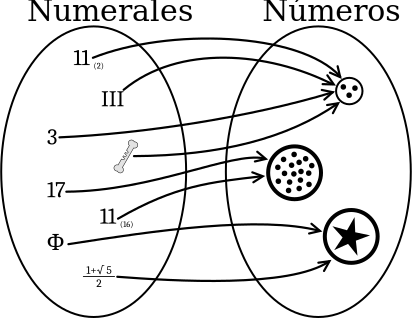
\includegraphics[height=0.65\textheight]{img/numerales.pdf}
        %\captionsetup{textfont=tiny,labelformat=empty,justification=centering}
        %\caption{}
    %\end{figure}

\end{frame}

\begin{frame}[label=temario]

    \frametitle{Temario}

\begin{itemize}
    \item Enteros:
    \begin{itemize}
        \item Sin signo \emph{(SS)}.
        \item Signo Magnitud \emph{(SM)}.
        \item Complemento a 2 \emph{(C2)}.
        \item Exceso.
    \end{itemize}
\end{itemize}
\end{frame}

\begin{frame}{Representación de enteros}
    \framesubtitle{Sistemas de representación}
    \begin{itemize}
        \item Es la forma en la que interpretamos un conjunto de \emph{bits}.
        \item Solamente se puede operar entre datos representados con el mismo
            sistema de representación.
        \item El resultado de toda operación vuelve a estar representado en el
            mismo sistema.
    \end{itemize}
\end{frame}

\begin{frame}{Representación de enteros}

    \framesubtitle{Representación de enteros sin signo \emph{(SS)}}

    Representación de números enteros positivos y el cero.

    \begin{itemize}
        \item Para representar cada número usamos su representación binaria,
            completando con ceros a la izquierda para utilizar todos los
            \emph{bits}.
        \item Con $k$\bit{} podemos representar $2^{k}$ números distintos.
        \item Como queremos incluir el cero (y queremos representar todos los
            enteros en el rango) el último número no puede ser $2^{k}$, sino
            $(2^{k})-1$.
        \item Por lo tanto el \emph{Rango de Representación (RR)} de los
            enteros sin signo con $k$\bit{} es $[0,(2^{k})-1]$.
    \end{itemize}
\end{frame}

\begin{frame}{Representación de enteros}

    \framesubtitle{Suma de enteros sin signo \emph{(SS)}}

    La suma de enteros sin signo en binario es muy similar a la suma en
    decimal. Solo hay que recordar las siguientes reglas:
    \pause
    \begin{itemize}
        \item Si no tenemos acarreo o el acarreo es cero:
            \begin{itemize}
                \item $0 + 0 = 0$, y no generamos acarreo.
                \item $1 + 0 = 1$, y no generamos acarreo.
                \item $1 + 1 = 0$, y generamos 1 de acarreo.
            \end{itemize}
        \pause
        \item Si tenemos 1 de acarreo:
            \begin{itemize}
                \item $(1) + 0 + 0 = 1$, y no generamos acarreo.
                \item $(1) + 1 + 0 = 0$, y generamos 1 de acarreo.
                \item $(1) + 1 + 1 = 1$, y generamos 1 de acarreo.
            \end{itemize}
    \end{itemize}
\end{frame}

\begin{frame}{Representación de enteros}
    \framesubtitle{Sistema de Signo-magnitud \emph{(SM)}}

    \begin{itemize}
        \item El \emph{bit} más significativo (el que esta más a la izquierda)
            representa el signo.
            \begin{itemize}
                \item \textbf{0 → Positivo}
                \item \textbf{1 → Negativo}
            \end{itemize}
        \item Los \emph{bits} restantes, el valor absoluto o magnitud.
        \item Si tenemos \emph{k}\bit, el \emph{RR} es:
            $[-(2^{k-1}-1),(2^{k-1})-1]$
    \end{itemize}\pause
    \emph{Ejemplo (con 8\bit{}):}
        \begin{itemize}
            \item $34_{10} = 0\, 0100010$
            \item $-34_{10} = 1\, 0100010$
        \end{itemize}
\end{frame}

\begin{frame}{Representación de enteros}
    \framesubtitle{\emph{(SM)}: Limitaciones}
    \begin{itemize}
        \item Doble representación del cero.
        \item No utiliza eficientemente los \emph{k}\bit{}.
        \item No es conveniente para la aritmética (poco práctico).
\end{itemize}
\end{frame}

\begin{frame}{Operación de Complemento a 2}
\begin{itemize}
    \item La operación de complementar a 2 consiste en obtener el opuesto de
        un número aritméticamente (el que tiene el mismo valor absoluto pero
        signo opuesto).
    \item $ C2(a) + a = 0 $
\end{itemize} \pause

    Para obtener el complemento a 2 de un número:
    
    \begin{itemize}
    \item Se invierte cada uno de los bits (reemplazando 0 por 1 y viceversa)
    \item Al resultado se le suma 1.
    \end{itemize}
    Ejemplo: $C2(1010) = 01011$
\end{frame}

\begin{frame}{Representación de enteros}
    \framesubtitle{Representación en Complemento a 2 \emph{(C2)}}

    Para representar un número \textit{a} en complemento a 2 con \emph{k}
    \textbf{bits}, comenzamos por considerar su signo:
    \begin{itemize}
    \pause
    \item Si \textit{a} es positivo o cero, lo representamos como en
        \emph{SS(k)}, es decir, lo escribimos en base 2 con \emph{k}\bit{}.
    \item Si \textit{a} es negativo, tomamos su valor absoluto, lo
        representamos como en \emph{SS(k)}, y le aplicamos la
            \textbf{operación} complemento a 2. 
\end{itemize}
\end{frame}

\begin{frame}{Representación de enteros}
    \framesubtitle{Representación en Complemento a 2 \emph{(C2)}}
    Ejemplo, representar 17 en \emph{C2} con \emph{k} = 8\bit{}:
    \pause
    \begin{itemize}
        \item $17_{10} = 0001\,0001_{2}$ con \textit{k} = 8 bits.
    \end{itemize}
    \pause
    Ejemplo, representar -17 en \emph{C2} con \emph{k} = 8\bit{}:
    \pause
    \begin{itemize}
        \item Buscamos la representación de $|-17|$:\\
        $17 = 0001\,0001_{2}$ con \textit{k} = 8 bits.
    \pause
        \item Aplicamos la operación de \emph{C2} a la representación de
            $|-17|$:\\
            $C2(0001\,0001) = 1110\,1111 = -17_{10}$
    \end{itemize}
\end{frame}

\begin{frame}{Representación de enteros}
    \framesubtitle{\emph{C2}: Rango de representación}
    El \emph{RR} del sistema de representación complemento a dos, con
    \emph{k}\bit{}, es:  $[-2^{k-1},(2^{k-1})-1]$ 
\end{frame}


\begin{frame}{Representación de enteros}
    \framesubtitle{Ventajas del sistema de representación \emph{C2} sobre
    \emph{SM}}

    \begin{itemize}
        \item El cero tiene una única representación, lo que facilita las
            comparaciones.
        \item No requiere comprobaciones de signo antes de operar. Se opera
            directamente.
        \item El mecanismo de cálculo es eficiente y fácil de implementar en
            hardware.
    \end{itemize}
\end{frame}

\begin{frame}{Error MUY frecuente}
    Para representar cualquier número en \emph{C2}... lo tengo que
    complementar a 2....  \textbf{NO!}
    \pause
    Al \textit{representar} en \emph{C2}, la \textit{operación} de
    complementar a 2 únicamente se aplica cuando queremos \textbf{obtener el
    opuesto de un número}.
\end{frame}

\begin{frame}{Representación de enteros}
    \framesubtitle{Aritmética en \emph{C2}}

    Una gran ventaja que aporta el sistema \emph{C2} es que no es
            necesario implementar algoritmos de resta: Cuando se necesita
            efectuar una resta, se complementa el sustraendo y luego se lo
            suma al minuendo.

    Las computadoras no restan: siempre suman.
\end{frame}

\begin{frame}{Desbordamiento (overflow)}
\begin{itemize}
    \item Cuando el resultado de una operación aritmética excede la cantidad de dígitos del sistema, el resultado es inválido.
    \item Es importante que la computadora lo detecte, para informar al proceso, y que pueda descartar el resultado.
\end{itemize}
\end{frame}


\begin{frame}{Desbordamiento en C2}
    \begin{itemize}
    \item Puede ocurrir tanto al sumar dos números positivos como dos negativos.
    \item Es fácil detectarlo en este sistema, observando los dos últimos bits de acarreo (carry).
    \end{itemize}
\end{frame}

\begin{frame}{Detectar desbordamiento en C2}
Se observan los dos últimos bits de acarreo (carry).
    \begin{itemize}
    \item Son diferentes? Hay overflow.
    \item Son iguales? No hay overflow.
\end{itemize}
\end{frame}

\begin{frame}{Detectar desbordamiento en C2}
    Ejemplo: 23 - 9 (extender el signo para llegar a los \textit{k} bits)
    \begin{itemize}
        \item 00010111 +
        \item 11110111
    \end{itemize}
\end{frame}

\begin{frame}{Detectar desbordamiento en C2}
    \begin{figure}
    \centering
    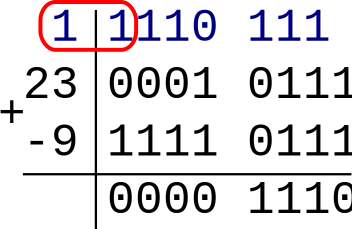
\includegraphics[height=0.75\textheight]{img/sumaSO.pdf}
    \captionsetup{labelformat=empty}
    \caption{}
    \end{figure}
\end{frame}

\begin{frame}{Detectar desbordamiento en C2}
    Ejemplo: 123 + 9
    \begin{itemize}
        \item 01111011 +
        \item 00001001
    \end{itemize}
\end{frame}

\begin{frame}{Detectar desbordamiento en C2}
    \begin{figure}
        \centering
        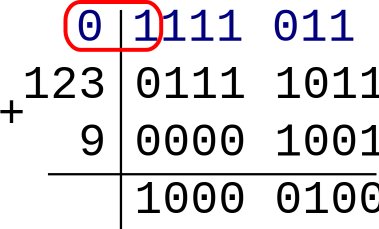
\includegraphics[height=0.75\textheight]{img/sumaCO.pdf}
        \captionsetup{labelformat=empty}
        \caption{}
    \end{figure}
\end{frame}

\begin{frame}{Notación en exceso}

    \begin{itemize}
    \item Se determina el intervalo de enteros a representar.
    \item Se determina la cantidad de bits necesarios para representar todos los enteros del intervalo.
    \end{itemize}
\end{frame}

\begin{frame}{Notación en exceso}
    \begin{itemize}
        \item Un intervalo de $[a,b]$ enteros, comprende \textit{n} valores, donde $n = b - a + 1$
        \item ¿Cuántos bits necesitamos para representar \textit{n} valores?
        \item Por ejemplo, para un intervalo $[150,157]$.
    \end{itemize}
\end{frame}

\begin{frame}{Notación en exceso}
    \begin{block}{Representar un intervalo de enteros}
    Notemos que tanto \textit{a} como \textit{b} pueden ser negativos. Así podemos representar intervalos arbitrarios de enteros, lo que nos vuelve a dar un sistema de representación con signo.
    \end{block}
\end{frame}

\begin{frame}{Notación en exceso}
\small Para saber qué número le corresponde a cada entero: $valor\_decimal - a$ 
    \begin{figure}
    \centering
    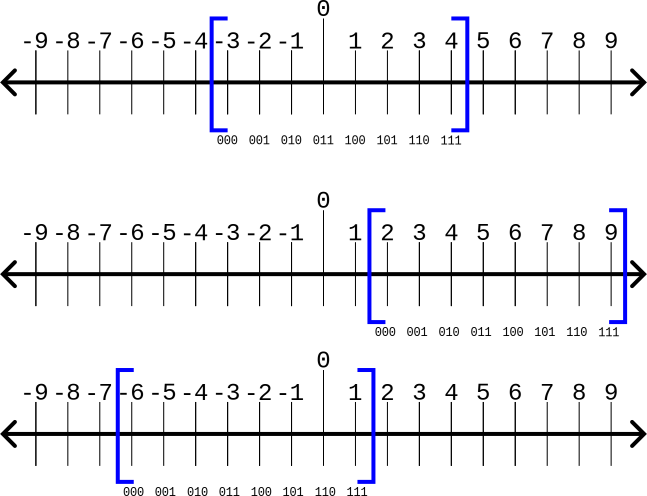
\includegraphics[width=0.75\textwidth]{img/exceso.pdf}
    \captionsetup{labelformat=empty}
    \caption{}
\end{figure}

\end{frame}

\againframe{temario}

\begin{frame}

\title{¿Consultas?}
\maketitle

\end{frame}

\newcounter{lastPage}
\setcounter{lastPage}{\number\value{page}}

\setcounter{page}{\number\value{lastPage}}

\end{document}
